\documentclass[a4paper, usesections, upjsfrontpage, disablespecwarning, thesismargins, thesislinespacing]{rnthesissvk}
\usepackage[slovak]{babel}
\usepackage[T1]{fontenc}
\usepackage[utf8]{inputenc}
\usepackage{graphicx}
\usepackage{caption}
\captionsetup[table]{name=Tab.}

\setcounter{secnumdepth}{4}

\title{Monitorovanie Informačných Systémov}
\author{Pavol Kozák}
\typprace{Bakalárska práca}
\pracovisko{Ústav informatiky}
\miesto{Košice}
\veduci{Doc. RNDr. Gabriel Semanišin PhD.}
\konzultant{RNDr. Erik Bruoth PhD.}
\rok{2015}

\podakovanie{Chcem sa poďakovať vedúcemu tejto práce Doc. RNDr. Gabrielovi Semanišinovi PhD., konzultantovi RNDr. Erikovi Bruothovi PhD. a Mgr. Slavomírovi Varchulovi za  cenné rady, odbornú pomoc a~konzultácie, ktoré mi poskytli pri vypracovaní tejto bakalárskej práce. \\ \\
Osobitné poďakovanie patrí mojej rodine a priateľom za podporu a pochopenie.}

\abstrakt{Hlavným cieľom našej bakalárskej práce je navrhnúť spôsob monitorovania informačného systému za účelom zbierania užitočných informácií ohľadom výkonu systému a používateľských preferenciách. Zaoberáme sa najmä otázkami aké informácie zbierať a akými nástrojmi ich zbierať. Existuje množstvo nástrojov z časti riešiacich našu problematiku. Zameriame sa na open-source nástroje. V práci si rozoberieme tie najpoužívanejšie, ich výhody a nevýhody a vybrané nástroje integrujeme do akademického informačného systému AIS2. Pomocou nich sa pokúsime zbierať a zobrazovať metriky, ktoré nám pomôžu identifikovať problémy a funkcie, ktoré je potreba vylepšiť.}

\begin{document}
\maketitle
\newpage

\setcounter{tocdepth}{3}
\tableofcontents

\newpage
\section{Úvod}

\subsection{Motivácia}

S informačnými systémami sa stretávame v dnešnej dobe čoraz častejšie. 
Mnohé systémy sa presúvajú z papierovej formy do elektronickej.
Môže to byť spôsobené mnohými výhodami tohto prechodu, ako napríklad jednoduchší prístup k informáciám, alebo len modernizáciou systému kvôli pokroku doby.

V tejto informačnej spoločnosti každý túži po informáciách.
S informačnými systémami sa stretávame na školách, na univerzitách, na pracoviskách, v zdravot\-níc\-tve a~v~rôznych iných oblastiach.

Vývojári informačných systémov sa snažia poskytnúť svojím zákazníkom informácie, ktoré hľadajú, kvôli ktorým navštívili ich informačný systém.
Aby vedeli, či ich systém funguje spoľahlivo, potrebujú ho nejakým spôsobom odmerať.

Na meranie systémov slúžia metriky.
Dávajú nám komplexnú informáciu o~systéme, o jeho nedostatkoch, o tom, čo vyžaduje zlepšenie, o rýchlosti a~spoľahli\-vos\-ti systému.
Pri zlepšovaní systému sú metriky veľmi užitočné.
Odhalia slabé miesta systému, ktoré by sme pri bežnom testovaní nespozorovali.

\subsection{Informačný Systém}

Informačný systém je zostavený z ľudí a počítačov, ktorý spracúvajú a interpretujú informácie.
Niekedy sa tento termín používa na označenie softvéru, ktorý využíva počítačovú databázu alebo len počítačového systému.
%\cite{website:wikipedia-informacnysystem}

V tejto práci sa budeme zameriavať na informačné systémy, ktoré sú vo forme webovej aplikácie.


\subsection{Web Aplikácia}

Webová aplikácia je aplikácia typu klient-server vytvorená pre prostredie internetu alebo intranetu.
V softvérovom inžinierstve je aplikácia poskytovaná užívateľom z~webového servera cez počítačovú sieť Internet, 
alebo jej vnútropodni\-kovú obdobu (intranet). 
Webové aplikácie sú populárne predovšetkým pre všade\-prítomnosť webového prehliadača ako klienta. 
Ten sa nazýva tenkým klientom, pretože sám o sebe logiku aplikácie nepozná.
Výhodou webových aplikácií je rovnaké užívateľské rozhranie kdekoľvek bez nutnosti inštalácie špeciálneho softvéru. 
Veľkou výhodou pre užívateľa ale aj pre prevádzkovateľa aplikácie je~jednoduchá aktualizácia. 
Tá sa vykonáva len na~jednom mieste - na serveri, na~ktorom webová aplikácia beží. Nevýhodou je nutnosť internetového pripojenia.
%\cite{website:wikipedia-webaplikacia}

\subsection{Metrika}
%http://epodnikanie.euin.org/node/126
Slovo metrika je často používaný pojem v oblasti monitorovania systémov.
Metri\-ky v oblasti monitorovania sú spôsoby a nástroje merania, vyjadrujú stav určitého systému, 
napríklad jeho kvality, efektívnosti a nadobúdajú pri tom rôzne hodnoty. 
Pri riadení sa používajú indikátory aj pre definíciu a dosahovanie cieľov prípadne ich žiaducich hodnôt. 
Používajú sa tiež špecializované pojmy Performance indicator alebo Key performance indicator.
%\cite{website:epodnikanie}
Metriky nám pomáhajú ‘‘odmerať’’ systém a tým nám dávajú komplexnú informáciu o systéme a pomáhajú odhaliť jeho slabé miesta.
Vhodne zvolené metriky dokážu nasmerovať vývojárov správnym smerom a poukázať na možné problémy a tým v konečnom dôsledku pomôžu zlepšiť monitorovaný systém.

\subsubsection{Rozdelenie Metrík}


Medzi základné delenia metrík patrí delenie na kvalitatívne a kvantitatívne metriky.
Kvantitatívne metriky udávajú číselnú hodnotu, zatiaľčo kvalitatívne metriky nečíselnú hodnotu.  
Kvantitatívne metriky sa ľahšie zobrazujú, interpretujú a sú zrozumiteľnejšie.
~\\
~\\
Metriky môžeme rozdeliť podľa druhu na:

\begin{itemize}
	\item výkonnostné metriky
	\item softvérové metriky
	\item aplikačné metriky
	\item systémové metriky
	\item používateľské metriky
\end{itemize}

V tejto práci nás budú zaujímať aplikačné, systémové a používateľské metriky.

\subsubsection{Aká je Dobrá Metrika?}

Aby metrika plnila svoj cieľ, teda podala správnu informáciu o systéme, mala by byť:
\begin{itemize}
	\item jednoduchá
	\item relevantná
	\item aktuálna
	\item okamžite ukončiteľná
\end{itemize}

Metrika by mala byť jednoduchá, aby bola ľahko interpretovateľná a pochopiteľná.
Relevantná metrika je taká, ktorá pomôže splniť cieľ, dosiahnuť to, na~čo~bola určená.
Neaktuálne metriky nám poskytnú neaktuálne, možno už~nep\-ravdivé dáta a preto by metriky mali byť aktuálne. 
Len aktuálne dáta nám popíšu systém spoľahlivo.
Od metriky požadujeme, aby bola okamžite ukončiteľná, aby hneď po jej získaní bola pripravená na spracovanie a tak viedla k novým poznatkom.
%\cite{website:web-analytics.wikidot}

\subsubsection{Typy Metrík}

Medzi základné typy metrík patria údaje o počte (counting), údaje o čase (timing), iné číselné hodnoty (celočíselné alebo desatinné), alebo niekedy aj nečíselné hodnoty (gauges). 

Údajmi o počte môžeme získavať metriky ako napríklad počet požiadaviek, ktoré prišli na server za nejaký časový interval, počet volaní metódy v kóde, počet kliknutí na tlačidlo v informačnom systéme. Metriky tohto typu zbierame inkrementovaním počítadla v nástroji ako metrics alebo statsd v klientskej časti.

Často potrebujeme zmerať časový údaj ako napríklad čas pripojenia k databáze, čas obsluhy požiadavky alebo čas strávený vykonávaním určitého kusu kódu. Zmeraný čas zaznamenáme nástrojom na zbieranie metrík.

Niekedy je užitočné zbierať hodnotu, ktorá nezávisí od predchádzajúcich hodnôt napríklad počet objektov v rade, veľkosť dát odoslanej odpovede, alebo zaťaženie procesora. 
Tieto hodnoty môžu byť číselné alebo nečíselné. Tieto hodnoty pravidelne zbierame a odosielame na spracovanie a zobrazenie.

\subsection{Monitorovanie Ais2}

V našej bakalárskej práci chceme navrhnúť systém monitorovania akademického informačného systému AIS2.
Problémom je to, že vývojári systému AIS2 nie sú správcami systému.
Nemôžu preto získavať metriky ako napríklad zaťaženie serverov, voľná operačná pamäť, či iné systémové metriky.
Aby zabezpečili hladký chod systému, musia sa spoľahnúť na aplikačné metriky.
Tie nám daju informácie o aktuálnom stave aplikácie a o jej správaní.

Keďže systém AIS2 beží vo viacerých inštaláciách, 
	je potrebné monitorovať viacero inštalácií tohto systému samostatne, aj ako celok.
Chceme ich vedieť porovnať medzi sebou, 
	aby sme vedeli odlíšiť problémy v konkrétnej inštalácii a globálne problémy týkajúce sa systému samotného.
Na porovnanie inštalácií potrebujeme získané metriky mať na jednom mieste, na jednom serveri, čo môže výrazne skomplikovať zber metrík.
Potrebujeme zobrazovať agregované metriky zo všetkých inštalácií.
Bude jednoduchšie inštalácie porovnať a analyzovať nazbierané metriky.

Ďalším cieľom monitorovania AIS-u je optimalizácia interakcie systému s používateľom.
Chceme detekovať zle navrhnuté dialógy, ich neprehľadné umiestnenie v systéme, a analyzovať interakciu s používateľmi, napríklad aj dynamickým upravovaním používateľského rozhrania.

\subsection{Problémy}

Hlavným cieľom monitorovania informačného systému je identifikovať problémy skôr ako používateľ.
Ak zbadá problém používateľ, už je neskoro.
Medzitým, ako nahlási problém vývojárom informačného systému, tento problém už mohlo zaznamenať množstvo ďalších používateľov.
Vývojári potom musia rýchlo problém identifikovať a opraviť, čo môže byť netriviálna záležitosť.
Ak by sme problém zaznamenali hneď ako nastane, mali by sme viac času na jeho riešenie.

Problém môže nastať, ak máme metrík veľa.
Monitorovanie systému nesmie systém výrazne zaťažiť, lebo by monitorovanie nebolo efektívne.

\subsection{Ilustračný Príklad}

Dobrým príkladom informačného systému je akademický informačný systém.
Monitorovanie takéhoto systému môže výrazne pomôcť k jeho vylepšeniu a~rozví\-janiu.

Ak by mal vývojár informáciu o prehliadačoch, ktorými sa používatelia pripojili do~systému, vedel by sa lepšie rozhodnúť, ktoré prehliadače má podporovať, aby pokryl čo najväčšiu skupinu používateľov.

Zaujímavou metrikou je aj rozlíšenie obrazoviek klientov, lebo s takouto informáciou sa dá lepšie rozvrhnúť používateľské rozhranie a zabezpečiť, aby klienti našli informácie, ktoré potrebujú rýchlejšie.
Ak by napríklad väčšina používateľov systému k nemu pristupovala s malou obrazovkou cez mobilný telefón, vývojár by investoval viac času a prostriedkov do prispôsobenia rozhrania pre mobilné telefóny.


\subsection{Prehľad Súčasného Stavu}

V tomto čase je množstvo informačných systémov, ktoré sú neustále vylepšované a~zdokonaľované a~tak je potreba ich monitorovať, aby sa dali ešte viac zlepšiť a~prispôsobiť zákazníkom.
Každý systém je špecifický, a tak aj jeho monitorovanie je jedinečné.
Vývojári sa snažia upraviť monitorovanie ich systému a prispôsobiť ho tak, aby im poskytol čo najviac vedomostí o ich systéme.

Existuje niekoľko nástrojov, ktoré ponúkajú riešenia načich problémov či už ide o zbieranie metrík alebo ich vizualizáciu.
Patria tu jak platené (Datadog, Stackdriver, Librato), tak aj open-source nástroje (Statsd, Metrics, Cacti, Graphite, Zabbix, Ganglia, Naggios).
My sa zaoberáme open-source nástrojmi.

\subsection{Ciele Práce}

\begin{enumerate}
	\item Navrhnúť spôsob monitorovania informačného systému v reálnom čase za~úče\-lom zhromažďovania informácií o výkonne systému a používateľských pre\-ferenciách.
	\item Navrhnúť dátovú štruktúru pre uložené metriky z jednotlivých inštalácií a~vytvoriť jednoduché štatistické prehľady nad zozbieranými údajmi v závis\-losti od~charakteru údajov.
	\item Analyzovať možnosti využitia monitorovania pre účely optimalizácie interakcie s používateľom.
\end{enumerate}

\newpage

%\section{Návrh Riešenia}

%\subsection{Úvod k zberu metrík}

\section{Algoritmus monitorovania informačného systému}

Ak chceme získať užitočné dáta o systéme aby sme ich mohli analyzovať, musíme ich najprv zozbierať.
Pred zbieraním metrík si treba najprv dobre premyslieť, čo chceme zbierať, 
aké metriky sú pre nás vhodné a aký cieľ chceme zberom metrík dosiahnuť.
Treba si dobre a jasne definovať metriky, aby sme z~nich mali čo najväčší osoh.

%\section{Algoritmus monitorovania informačného systému}

Monitorovanie informačného systému od prípravy na monitorovanie až po analýzu výsledkov monitorovania sa dá popísať nasledujúcim algoritmom:

\begin{enumerate}
	\item Určenie cieľov monitorovania informačného systému.
	\item Výber vhodných metrík.
	\item Výber nástrojov na monitorovanie a zobrazovanie metrík.
	\item Integrácia nástrojov a metrík do informačného systému.
	\item Samotný zber metrík.
	\item Analýza získaných metrík.
	\item Vyvodenie dôsledkov monitorovania.
\end{enumerate}

Určenie cieľov monitorovania informačného systému je dôležité.
Musíme si dobre premyslieť, na čo chceme monitorovanie zamerať, čo chceme zlepšiť, čo potrebujeme odmerať.
Taktiež je dôležité premyslieť si, čo urobíme s výsledkom monitorovania a nakoľko bude výsledok merania relevantný a pravdivý.
To závisí aj od metrík, ktoré si zvolíme, od času a obdobia, v ktorom systém budeme monitorovať.
Treba si ujasniť problémy, ktoré chceme vyriešiť pomocou monitorovania.

Na to, aby sme monitorovaním dosiahli stanovené ciele, musíme si zvoliť vhodné metriky, 
	ktoré nám poskytnú odpovede na naše otázky.
Každý systém je odlišný a tak neexistuje univerzálny návod, aké metriky si zvoliť.
Treba sa zamyslieť nad tým, aké údaje by nám pomohli, keby sme ich mali k dispozícii.
Ak potrebujeme získať informácie o používateľoch a o ich správaní v systéme, pomohli by nám používateľské metriky.
Ak potrebujeme získavať údaje o stave aplikácie, potom je pre nás vhodné zbierať aplikačné metriky.
Keď chceme zistiť, aký je výkon systému a ako sa správa systém pri zaťažení a pod akou záťažou je v konkrétnych obdobiach, potom by sme sa mali zamerať na systémové metriky.

Ak už máme definované metriky, ktoré chceme zbierať, v ďalšej časti prípravy na monitorovanie si zvolíme vhodné nástroje na zber 	metrík a na ukladanie a zobrazovanie metrík.
Môžeme si zbieranie, ukladanie a zobrazovanie metrík navrhnúť a implementovať aj posvojom, ale keďže je monitorovanie informačných systémov rozšírené, existujú už špecializované nástroje, ktoré nám pomôžu s monitorovaním a zabezpečia nám kompatibilitu s ďalšími nástrojmi.
Nástrojov ktoré máme k dispozícii je niekoľko.
V Tejto práci si rozoberieme open-source nástroje na zbieranie metrík Statsd a Metrics a nástroje na zbieranie metrík Graphite, Zabbix a Ganglia.
Všetky nástroje sú odlišné a majú svoje výhody a nevýhody, ktoré si podrobnejšie popíšeme.
Nástroje si vyberieme podľa funkcionality, náročnosti integrácie a podľa veľkosti informačného systému.

Po výbere nástrojov na monitorovanie nasleduje integrácia vybraných nástrojov a metrík do systému.
Zložitosť integrácie a konfigurácie závisí od nástrojov, ktoré sme si zvolili a od komplexnosti monitorovaného systému.
Metriky zbierame v podobe counterov, timerov a gauges, prípadne im podobným alebo inak pomenovaným alternatívnym spôsobom podľa vybraných nástrojov.

Ak máme nakonfigurované nástroje na zber metrík a funkčné prepojenie nástroja na zber metrík s nástrojom na ukladanie a zobrazovanie metrík, nasleduje fáza samotného zbierania metrík a monitorovania informačného systému.
V tejto fáze sledujeme metriky, ktoré nám nástroj na zobrazovanie metrík vykresľuje v prehľadných grafoch.
Niektoré zobrazovacie nástroje umožňujú aj agregáciu grafov pre jednotlivé metriky, to znamená, že súvisiace metriky si zobrazíme v jednom spoločnom grafe. 

Niektoré nástroje, alebo ich jednoduché prepojenie s ďalším nástrojom ponúkajú možnosť notifikácie administrátora o udalostiach, ktoré nastali v systéme.
Môžeme tak byť notifikovaný napríklad o priveľkej záťaži na systém, o nedostatku voľnej operačnej pamäti alebo o pridlhom čase čakania klienta na odpoveď zo servera.
To nám pomôže identifikovať aktuálne nastávajúci problém, ktorý je potrebné čo najskôr vyriešiť.
Takisto nám to pomôže odhaliť problém skôr, ako ho odhalý používateľ nášho systému.

Ak už zbierame metriky dlhšiu dobu, máme dostatok údajov na ich analýzu a ďalšie spracovanie.
Môžeme analyzovať, ako sa systém správa v určitých obdobiach, ako sa správajú používatelia v systéme a ako sa správa systém, keď je pod záťažou. To nám pomôže pripraviť sa na ďalšiu záťaž, alebo zistíme, že potrebujeme zbierať ďalšie metriky, na ktoré sme na začiatku nemysleli, alebo sa nám zdali irelevantné.

V ďalšej fáze vyvodíme dôsledky monitorovania.
Zamyslíme sa, či nám monitorovanie pomohlo splniť ciele, ktoré sme si na začiatky stanovili a ako nám to pomohlo zlepšiť systém.
Porozmýšľame, čo nám ešte treba zlepšiť, aké závery nám plynú z monitorovania a určíme ďalšie kroky k ešte lepšiemu monitorovaniu.
Monitorovanie informačného systému je dlhodobý proces, a počas monitorovania sa môže meniť a upravovať s meniacím sa systémom a už získanými poznatkami z monitorovania.
Môžeme pridávať nové metriky aj s novou funkcionalitou alebo tie nepodstatné metriky zmazať.
V tejto fáze upravíme systém podľa výsledkov, ktoré sme získali monitorovaním.
Napríklad ak sme zistili, že náš systém potrebuje optimalizáciu dopytov do databázy, optimalizujeme ich a sledujeme, aký to ma dopad na systém a na rýchlosť odpovede na požiadavky od klientov.

Na obrázku 1. môžete vidieť diagram algoritmu pre monitorovanie informačného systému.

\begin{figure}
\begin{center}
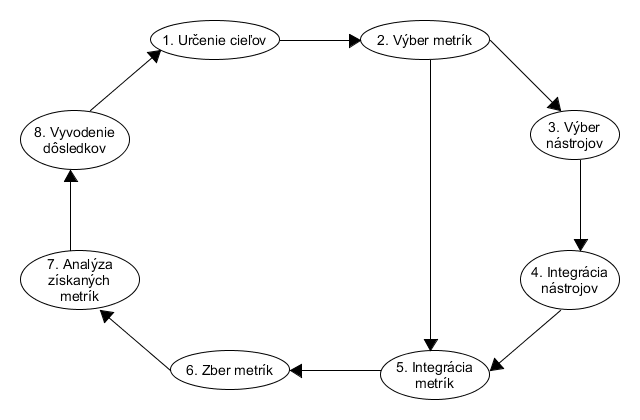
\includegraphics[scale=0.41]{ais_algorithm.png}
\caption{Diagram algoritmu pre monitorovanie informačného systému}
\end{center}
\end{figure}

\newpage

\section{Typy monitorovania}

\subsection{Zber metrík v reálnom čase}

Monitorovanie systému v reálnom čase nám pomôže detekovať problém skôr, ako ho zbadá používateľ.



\subsection{Dlhodobé zbieranie metrík}

Krátkodobé merania systému nám podajú užitočnú informáciu o aktuálnom stave systému a o jeho používateľoch.
Nás však zaujímajú aj dlhodobé merania.
Tie nám povedia, kedy v priebehu roka je systém najviac zaťažený, kedy najmenej, a aké funkcionality používatelia využívajú v konkrétnych obdobiach.
To sa nám pomôže pripraviť na najväčšiu záťaž.

% TODO dopisat novu funkcionalitu

\subsection{Zbieranie metrík za účelom hľbkovej analýzy}

Dlhodobými meraniami vieme zaznamenávať vzory správania používateľov v našom informačnom systéme.
Takýmto vzorom môže byť v akademickom informačnom systéme napríklad:

\begin{itemize}
	\item Používatelia si najčastejšie po prihlásení do aplikácie prečítajú nové správy.
	\item Po prečítaní správ sa odhlásia alebo:
	\begin{itemize}
		\item Ak je začiatok semestra, pozrú si rozvrh hodín.
		\item Ak je stred semestra, pozrú sa na priebežné hodnotenie.
		\item Ak je koniec semestra, prihlásia sa na skúšku.
	\end{itemize}
\end{itemize}

Ak získame takéto vzory, môžeme napríklad dynamicky meniť používateľské rozhranie počas priebehu semestra a sprístupniť tak najčastejšie hľadané informácie podľa vzorov na viditeľnejšie miesta v našom systéme.

% TODO zle navrhnuté dialógy

\newpage

\section{Nástroje na Zber Metrík}

Ak už máme jasne definované metriky, môžeme ich začať zbierať.
Zber metrík je~často riešený problém, v zbere metrík nám môžu pomôcť rôzne nástroje.
Medzi naj\-populár\-nejšie open-source nástroje na zber metrík patria Metrics a Statsd.
Sú to nástroje určené na odosielanie nameraných metrík do nástrojov na uloženie a zobrazenie metrík v podobe grafov.

Integrácia oboch nástrojov si však vyžaduje určité zmeny v kóde systému.
Každý systém je jedinečný a teda aj jeho monitorovanie je odlišné.
To si však žiada odlišné metriky a tie sa zbierajú na odlišných miestach v kóde systému.

Obe nástroje sú odlišné z hľadiska integrácie a architektúry.
Naším čiastočným cieľom je porovnať ich.
V nasledujúcich odstavcoch si popíšeme ich výhody a nevýhody.

\subsection{Nástroj Metrics}

Metrics je open-source java knižnica na zber metrík.
Získané metriky posiela do nástrojov na zobrazovanie metrík ako napríklad Graphite alebo Ganglia, alebo ukladá do databázy prostredníctvom logovacích nástrojov.

Keďže Metrics je java knižnica, integrácia nástroja do java webovej aplikácie je~záležitosť pridania niekoľkých závislostí.
Následne definujeme registre, v ktorých budú metriky uložené.
Ďalej je potrebné nastaviť reportovanie do ďalších nástrojov.
Potom na vhodných miestach v aplikácii získame metriky pomocou counterov, timerov a gauges, ktoré chceme zbierať.
Nástroj Metrics nám pomôže dostať namerané metriky do~ďalších nástrojov.

Asi najväčšou konkurenciou k Metrics je nástroj Statsd.


\subsection{Nástroj Statsd}

Open-source nástroj Statsd je určený na zber metrík a následné preposlanie do nástrojov na spracovanie a zobrazenie.
Má kientov pre množstvo programovacích jazykov ako napríklad node.js, java, python, ruby, perl, php, c, cpp, .net, či dokonca plugin pre wordpress. 

Statsd klient posiela získane metriky na oddelený statsd server, ktorý ich prijíma, akumuluje a v nastavených časových intervaloch odosiela do ďalších nástrojov. 
Slúži ako rýchla cache pre metriky. 
Umožňuje posielať dáta do nástrojov ako napríklad Graphite, Ganglia, Librato, Zabbix, či Mongo, Mysql, Datadog a mnoho ďalších.

Architektúra tohto nástroja je trochu zložitejšia.


\subsection{Metrics vs Statsd}

Obe nástroje slúžia na zbieranie metrík, majú však rozdielnú architektúru. 
Ponúkajú rôzne možnosti integrácie s ďalšími nástrojmi. 
Kvôli prehľadnosti sú základné rozdiely popísané v tabuľke 1.

\begin{table}
	\caption{Porovnanie nástrojov Metrics a Statsd}
	\centering
	\begin{tabular}{| p{3.7cm} | p{4.5cm} | p{4.7cm} |}
		\hline\noalign{\smallskip}
		Atribút porovnania & Metrics & Statsd \\
		\noalign{\smallskip}
		\hline
		Architektúra & Server totožný s klientom & Server a klient oddelený \\ \hline

		Integrácia s ďalšími nástrojmi & Ganglia, Graphite, Librato, Spring, Sematext, Wicket, Guice, Scala, Clojure, Cassandra, 	Elasticsearch, Statsd, Datadog, Influxdb, Cdi, Aspectj, Apache Camel & Amqp, Ganglia, Librato, Socket.io, Statsd, Mongo, Mysql, Datadog, Monitis, Instrumental, Hosted graphite, Zabbix, Opentsdb, Influxdb, Stackdiver, Couchdb \\ \hline

		Implementácia Servera & Iba Java & Node.js, Python, Ruby, C, Go, Clojure, 	Perl \\ \hline

		Implementácia Klienta & Klient totožný so serverom & Node.js, Java, Python, Ruby, Perl, Php, Clojure, C, Cpp, .Net, Go, 	Apache, Io, Varnish, PowerShell, JavaScript, Cocoa, ActionScript, Wordpress \\ \hline

		Licencia & Apache 2 & MIT \\ \hline

		Zložitosť integrácie do java web aplikácie & Import knižnice, definovanie metrík, nastavenie reportovania & Inštalácia Node.js, Statsd servera, import Statsd klientskej knižnice, definovanie metrík, inštalácia reportovacích backendov, konfigurácia Statsd servera \\ \hline

		Počet prispievateľov & 127 & 154 \\ \hline

		Počet releasov & 51 & 11 \\ \hline

		Prvý commit do repozitára & 27.4.2011 & 30.12.2010 \\ \hline
		
		Počet commitov do repozitára & 1958 & 823 \\ \hline

		%Dokumentácia & Dostatočná & Dostatočná \\ \hline
	\end{tabular}
\end{table}

\newpage

\section{Nástroje na Ukladanie a Zobrazenie Metrík}

Keďže monitorovanie informačných systémov je populárne, existujú rôzne nástroje na~ukladanie a zobrazenie metrík.
Niektoré z nich sú komerčné, iné open-source.
Medzi často používané open-source nástroje patria nástroje Graphite, Zabbix a Ganglia.
Tieto nástroje vedia prijať dáta z iných nástrojov, uložiť ich v databáze a~vhodným spôsobom ich zobraziť, aby sa dali ľahšie interpretovať.
Metriky sa zobrazujú v podobe histogramov alebo čiarových diagramov cez používateľské rozhranie vo forme webovej aplikácie.

\subsection{Nástroj Graphite}

Nástroj Graphite je veľmi obľúbeným nástrojom v oblasti zobrazovania metrík.
Nástroje ako napríklad Statsd alebo Metrics pošlú získané metriky do Graphitu a ten ich uloží pomocou integrovaného nástroja Carbon do Whisper databázy. 
Whisper databáza je veľmi podobná RRD (round robin database) databáze, ale je prispôsobená a~napísaná v pythone.
Kód graphitu je napísaný v programovacom jazyku python.
Metriky stačí poslať do nástroja Graphite a on ich sám zaradí do stromu metrík podľa prefixu.
Po inštalácii sa nevyžaduje žiadna dodatočná konfigurácia.

Na obrázku 1 môžete vidieť používaťeľské rozhranie nástroja graphite a čiarový diagram pre metriku zaťaženie procesora.

\begin{figure}
\begin{center}
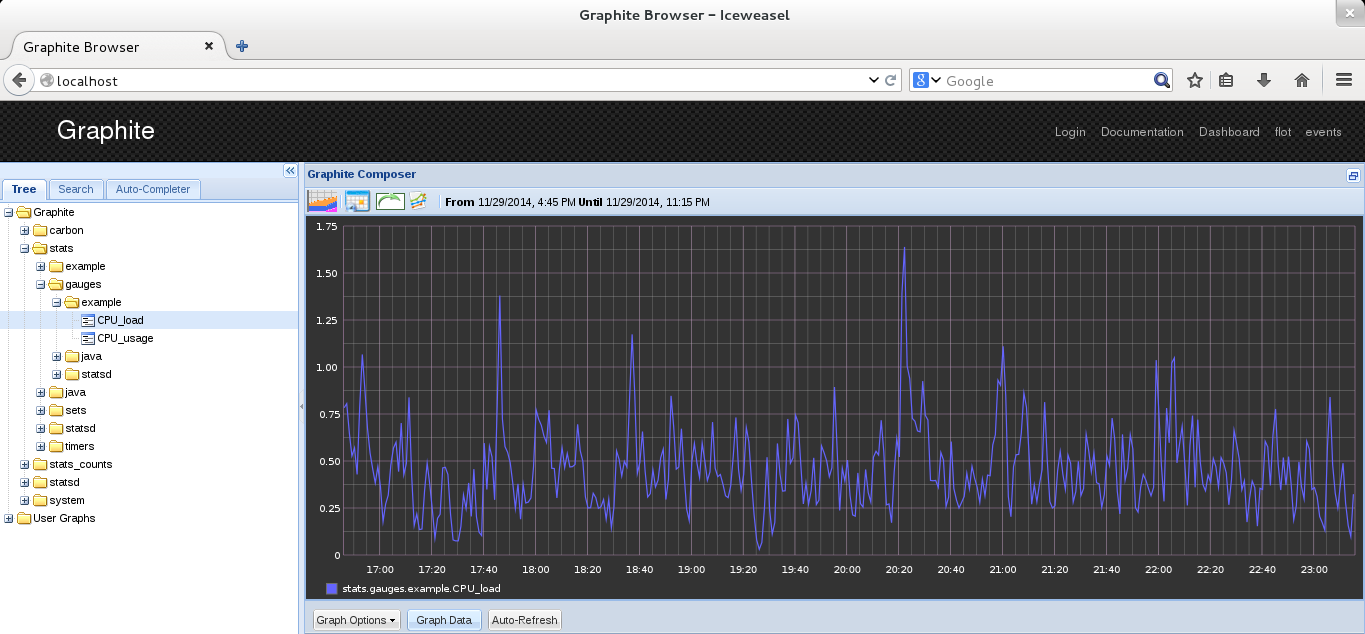
\includegraphics[scale=0.41]{graphite1.png}
\caption{Používateľské rozhranie nástroja Graphite}
\end{center}
\end{figure}

Nástroj Graphite je jednoduchý open-source nástroj určený na ukladanie a zobrazovanie metrík v podobe grafov.
Na vykresľovanie grafov využíva python knižnicu PyCairo.
V praxi sa používa pri jednoduchých projektoch, ak nám postačuje získané metriky zobrazovať.
Pri monitorovaní komplexnejších systémov sa používajú zložitejšie nástroje ako napríklad Zabbix alebo Ganglia.

\subsection{Nástroj Zabbix}

Ďalším používaným nástrojom je Zabbix.
Jeho kód je napísaný v jazyku C a~používateľské rozhranie v podobe webovej aplikácie je napísaný v jazyku PHP.
Na ukladanie metrík používa Mysql databázu.
Na obrázku 2 môžete vidieť používateľské rozhranie nástroja Zabbix.

\begin{figure}
	\begin{center}
		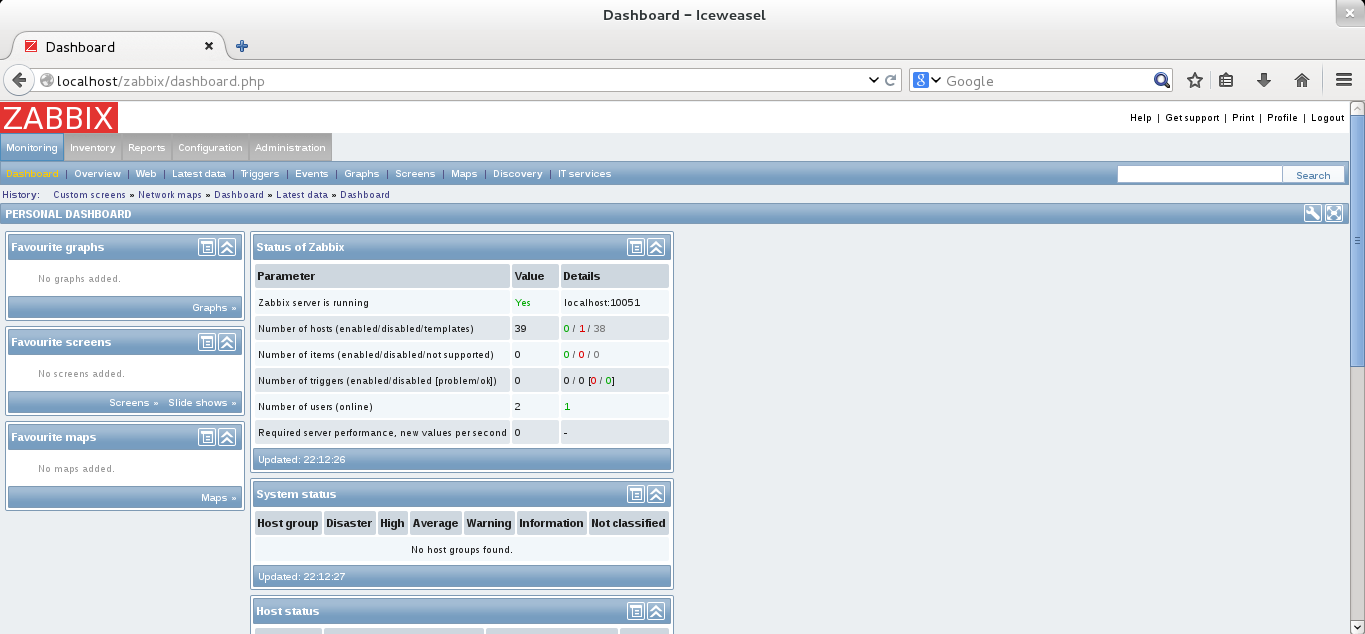
\includegraphics[scale=0.41]{zabbix.png}
	\end{center}
	\caption{Používateľské rozhranie nástroja Zabbix}
\end{figure}

Zabbix okrem vizualizácie dokáže zbierať vlastné metriky, pomáha detekovať problém a vie o ňom notifikovať administrátorov.
Je to omnoho mohutnejší nástroj ako Graphite.

K informačnému systému patrí aj hardvér, na ktorom systém beží.
Informácie o hardvéri a rôzne systémové metriky môžeme zbierať pomocou Zabbixu.
Môžeme monitorovať napríklad výkon systému, sieťové zariadenia, virtuálne stroje, databázy, Java virtual machine alebo Java aplikačné servery.

Zbieranie dát umožňuje napríklad Zabbix agent, ktorý pravidelne posiela získané udaje zo stroja, kde je nasadený na Zabbix server.
Zabbix tiež umožňuje na zber dát použiť SNMP a IPMI agentov alebo Zabbix sender nástroj, ktorým do Zabbixu vieme poslať ľubovoľné metriky.
Každá metrika, ktorá je poslaná do Zabbixu musí byť dopredu nakonfigurovaná.

Detekcia problému funguje pomocou definovania triggerov, ktoré odhalia, že niečo nefunguje.
Môže to byť napríklad výpadok stroja, málo voľného miesta na disku monitorovaného zariadenia alebo veľa pripojených používateľov.

Ak Zabbix detekuje problém, môže nás o tom notifikovať alebo vykonať požadovanú akciu.
Môže nás notifikovať prostredníctvom e-mailu, SMS správy alebo správy cez Jabber.
Môžeme si nastaviť, aké dáta sa nám v notifikácii zobrazia.
Okrem notifikačnej správy Zabbix vie po detekcii problému vykonať napríklad shell príkaz cez~ssh.

\subsection{Nástroj Ganglia}

Dalším obľúbeným nástrojom je Ganglia.
Ganglia je open-source nástroj zameraný na~distribuované monitorovanie celých clustrov či gridov.
Je naozaj rozšírený, používajú ho napríklad známe spoločnosti ako Twitter, flickr, National Aeronautics and Space Administration (NASA), Wikipedia, CERN, Cisco, HP, Microsoft, Dell, nVidia, U.S. Air Force.

Metriky do Ganglie môžeme poslať pomocou Gmond modulov, gmetric modulu alebo inými nástrojmi, ako napríklad statsd.
Ak posielame metriky do Ganglie, nemusíme ich mať dopredu nakonfiguroavné.
Gmetad vytvorí nový RRD súbor pre každú novú metriku, čo značne uľahčí konfiguráciu, ak metrík máme veľa.
Web používaťeľské rozhranie potom zobrazí základný graf pre každú metriku.

Ganglia na posielanie metrík na centrálny server používa dvoch démonov a to gmond a gmetad.
Gmond môže posielať alebo prijímať metriky, ktoré si drží v pamäti.
Gmetad v rámci gridu ťahá dáta z jedného gmond démona v rámci gridu.
Gmond moduly so sebou komunikujú cez UDP, do Gmetad posielajú XML cez TCP.
Gmetad si medzi sebou posielajú metriky cez TCP vo forme XML.
Gmond medzi sebou kominikujú buď unicastom alebo multicastom.
Architektúra je popísaná na obrázku 3.

\begin{figure}
	\begin{center}
		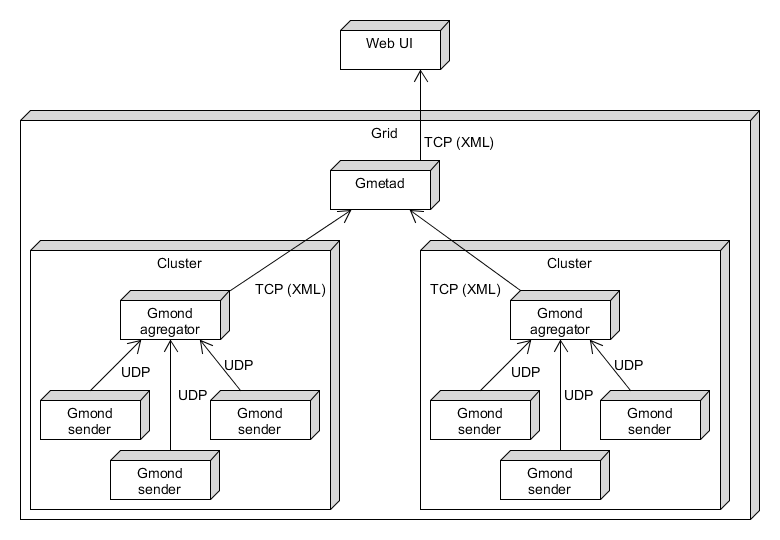
\includegraphics[scale=0.55]{ganglia-architecture.png}
	\end{center}
	\caption{Posielanie metrík do Ganglie použitím unicastu}
\end{figure}

\begin{figure}
	\begin{center}
		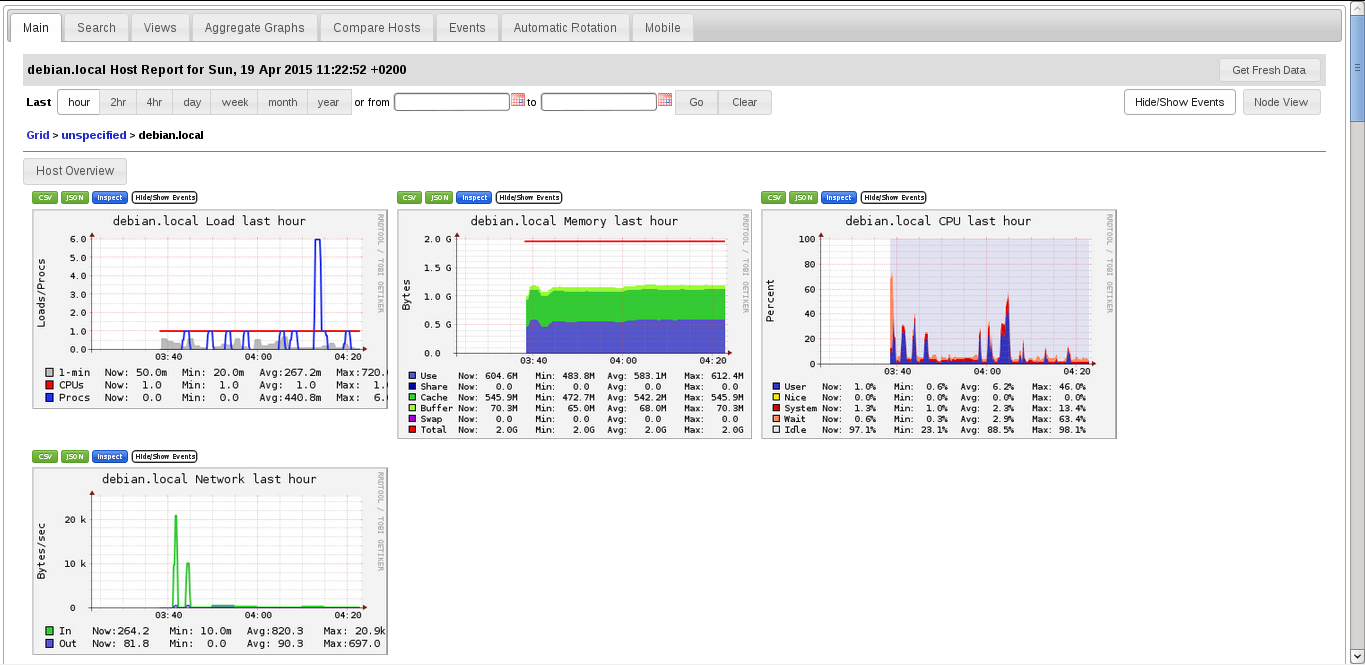
\includegraphics[scale=0.41]{ganglia.png}
	\end{center}
	\caption{Používateľské rozhranie nástroja Ganglia}
\end{figure}

\subsection{Graphite vs Zabbix vs Ganglia}

Ako sme už písali, nástroj Graphite je vhodný na monitorovanie menších systémov.
Pre väčšie informačné systémy je lepšie použiť komplexnejší nástroj, ako napríklad Zabbix alebo Gangliu.
Tie nám ponúkajú viac užitočných funkcií, ktoré môžeme využiť.
Zabbix vie detekovať problémy a tie jednoduchšie aj vyriešiť (napríklad reštartom zlyhanej služby), 
	Ganglia zas dokáže monitorovať celé clustre a gridy a ponúka nám jednoduchú agregáciu grafov.
Záleží od komplexnosti systému, ktorý nástroj si vyberieme.


\newpage

\section{Záver}

V tejto práci sme sa zaoberali monitorovaním informačných systémov, prečo je monitorovanie výhodné a ako nám môže pomôcť pri jeho rozvíjaní.
Rozobrali sme si open-source nástroje na zbieranie a vizualizáciu metrík a to Statsd, Metrics, Graphite, Zabbix a Ganglia.

%
\bibliography{bakalarka}

\renewcommand{\bibname}{Zoznam pou�itej literat�ry}
%\begin{thebibliography}{9}
%\bibitem{1} Ipsum, L.: Lorem ipsum dolor sit amet.
%\end{thebibliography}
%

\end{document}